\documentclass[12pt]{article}
\usepackage[margin=2.5cm]{geometry}
\usepackage{titling}
\usepackage{enumerate}
\usepackage{graphicx}
\usepackage{mdframed}
\usepackage{listings}
\usepackage{xcolor}
\usepackage{hyperref}
\usepackage[utf]{kotex}

\definecolor{codegreen}{rgb}{0,0.6,0}
\definecolor{codegray}{rgb}{0.5,0.5,0.5}
\definecolor{codepurple}{rgb}{0.58,0,0.82}
\definecolor{backcolour}{rgb}{0.95,0.95,0.92}

\lstdefinestyle{mystyle}{
    backgroundcolor=\color{backcolour},
    commentstyle=\color{codegreen},
    keywordstyle=\color{magenta},
    numberstyle=\tiny\color{codegray},
    stringstyle=\color{codepurple},
    basicstyle=\ttfamily\footnotesize,
    breakatwhitespace=false,
    breaklines=true,
    captionpos=b,
    keepspaces=true,
    numbers=left,
    numbersep=5pt,
    showspaces=false,
    showstringspaces=false,
    showtabs=false,
    tabsize=1
}

\lstset{style=mystyle}

\predate{}
\postdate{}

\begin{document}
\title{Lab 3: Inheritance}
\date{}
\maketitle

\section*{1) Play a game}

In this lab you’ll write code to play a simple number game:

\begin{itemize}
    \item This game can be played with two or more players.
    \item When the game starts, there is a count that begins at 0.
    \item On a player’s turn, they add to the count an integer that must be between a set minimum and a set maximum.
    \item The player whose move causes the count to be greater than or equal to a set goal amount is the winner.
\end{itemize}

\bigskip

\noindent Here’s a sample game with two players, where the goal is 21, the minimum move is 1, and the maximum move is 3. David is the winner.

\begin{center}
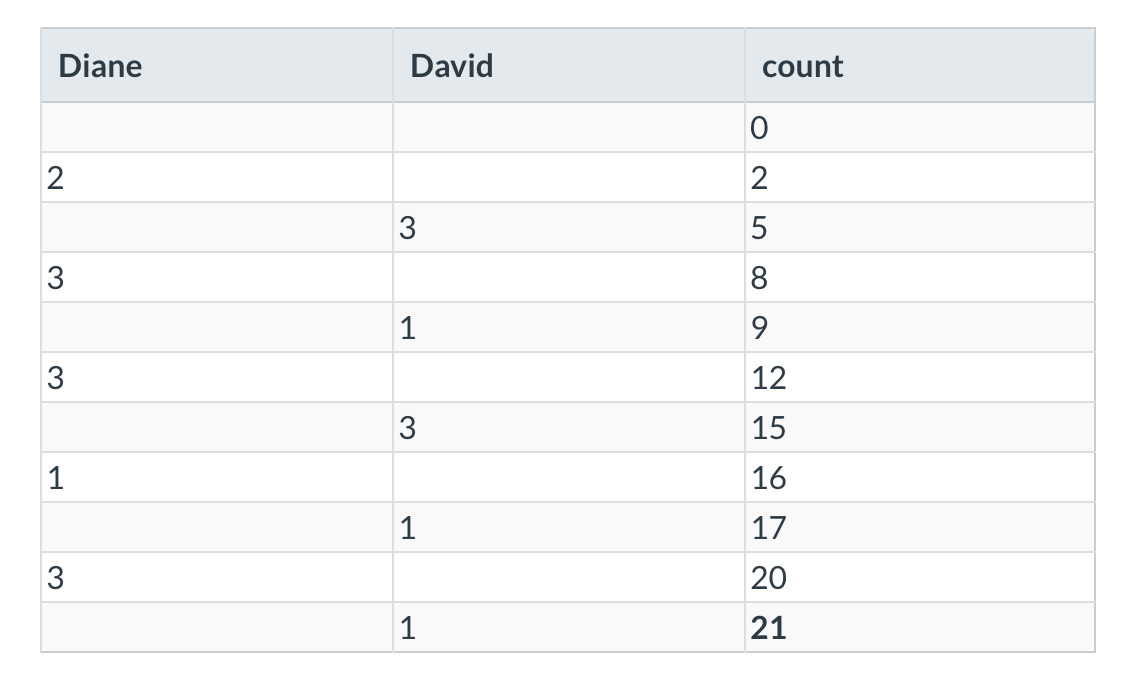
\includegraphics[width=0.8\linewidth]{../images/lab_3/table.png}
\end{center}

\bigskip

\noindent Play the game several times with your partner, using goal 21, minimum move 1,
and maximum move 3. Does a good strategy emerge?

\bigskip

\noindent (Even if it doesn’t, move on after a few minutes when you understand the game.
We’ll come back to strategies later.)

\section*{2) Become familiar with class \textit{NumberGame}}

\bigskip

Check module lab3.py the document into your lab3 folder.

\bigskip

\noindent Read the \textit{NumberGame} class carefully and answer the following questions
about it. Note that the entire class is provided for you, and your job here is
to understand it—in other words, you’re practicing your code reading skills.

\bigskip

\begin{enumerate}[1.]
    \item What attribute stores the players of the game?
    \item If \textit{turn} is 15, whose turn is it?
    \item Write a line of code that would create an instance of \textit{NumberGame}
    that violates one of the representation invariants.
    \item Which of the representation invariants is it possible to violate by
    constructing a \textit{NumberGame} improperly?
    \item List all the places in this class where a \textit{Player} is stored, an instance
    attribute of \textit{Player} is accessed or set, or a method is called on a \textit{Player}
\end{enumerate}

\bigskip

\begin{lstlisting}[language=Python,caption={lab3.py},captionpos=b]
    """CSC148 Lab 3: Inheritance

    === CSC148 Fall 2019 ===
    Department of Computer Science,
    University of Toronto

    === Module Description ===
    This module contains the implementation of a simple number game.
    The key class design feature here is *inheritance*, which is used to enable
    different types of players, both human and computer, for the game.
    """
    from __future__ import annotations
    import random
    from typing import Tuple


    class NumberGame:
        """A number game for two players.

        A count starts at 0. On a player's turn, they add to the count an amount
        between a set minimum and a set maximum. The player who brings the count
        to a set goal amount is the winner.

        The game can have multiple rounds.

        === Attributes ===
        goal:
            The amount to reach in order to win the game.
        min_step:
            The minimum legal move.
        max_step:
            The maximum legal move.
        current:
            The current value of the game count.
        players:
            The two players.
        turn:
            The turn the game is on, beginning with turn 0.
            If turn is even number, it is players[0]'s turn.
            If turn is any odd number, it is player[1]'s turn.

        === Representation invariants ==
        - self.turn >= 0
        - 0 <= self.current <= self.goal
        - 0 < self.min_step <= self.max_step <= self.goal
        """
        goal: int
        min_step: int
        max_step: int
        current: int
        players: Tuple[Player, Player]
        turn: int

        def __init__(self, goal: int, min_step: int, max_step: int,
                     players: Tuple[Player, Player]) -> None:
            """Initialize this NumberGame.

            Precondition: 0 < min_step <= max_step <= goal
            """
            self.goal = goal
            self.min_step = min_step
            self.max_step = max_step
            self.current = 0
            self.players = players
            self.turn = 0

        def play(self) -> str:
            """Play one round of this NumberGame. Return the name of the winner.

            A "round" is one full run of the game, from when the count starts
            at 0 until the goal is reached.
            """
            while self.current < self.goal:
                self.play_one_turn()
            # The player whose turn would be next (if the game weren't over) is
            # the loser. The one who went one turn before that is the winner.
            winner = self.whose_turn(self.turn - 1)
            return winner.name

        def whose_turn(self, turn: int) -> Player:
            """Return the Player whose turn it is on the given turn number.
            """
            if turn % 2 == 0:
                return self.players[0]
            else:
                return self.players[1]

        def play_one_turn(self) -> None:
            """Play a single turn in this NumberGame.

            Determine whose move it is, get their move, and update the current
            total as well as the number of the turn we are on.
            Print the move and the new total.
            """
            next_player = self.whose_turn(self.turn)
            amount = next_player.move(
                self.current,
                self.min_step,
                self.max_step,
                self.goal
            )
            self.current += amount
            self.turn += 1

            print(f'{next_player.name} moves {amount}.')
            print(f'Total is now {self.current}.')


    # TODO: Write classes Player, RandomPlayer, UserPlayer, and StrategicPlayer.


    def make_player(generic_name: str) -> Player:
        """Return a new Player based on user input.

        Allow the user to choose a player name and player type.
        <generic_name> is a placeholder used to identify which player is being made.
        """
        name = input(f'Enter a name for {generic_name}: ')
        # TODO: Create and return some sort of Player.


    def main() -> None:
        """Play multiple rounds of a NumberGame based on user input settings.
        """
        goal = int(input('Enter goal amount: '))
        minimum = int(input('Enter minimum move: '))
        maximum = int(input('Enter maximum move: '))
        p1 = make_player('p1')
        p2 = make_player('p2')
        while True:
            g = NumberGame(goal, minimum, maximum, (p1, p2))
            winner = g.play()
            print(f'And {winner} is the winner!!!')
            print(p1)
            print(p2)
            again = input('Again? (y/n) ')
            if again != 'y':
                return


    if __name__ == '__main__':
        # Uncomment the lines below to check your work using
        # python_ta and doctest.
        import python_ta
        python_ta.check_all(config={
            'extra-imports': ['random'],
            'allowed-io': [
                'main',
                'make_player',
                'move',
                'play_one_turn'
            ]
        })
        # import doctest
        # doctest.testmod()

        # Uncomment the following line to run the number game.
        # main()

\end{lstlisting}

\section*{3) Become familiar with function \textit{main}}

\bigskip

Now look at function \textit{main} and answer these question.

\begin{enumerate}[1.]
    \item Where is a \textit{NumberGame} constructed?
    \item This function calls \textit{g.play} repeatedly in a loop. What about the
    game can change each time \textit{g.play} is called: the goal, the min or max
    move, the players, the moves?
    \item List all the places in this function where a \textit{Player} is stored,
    an instance attribute of \textit{Player} is accessed or set, or a method is
    called on a \textit{Player}.
\end{enumerate}

\bigskip

\section*{4) Plan a Player class and 3 subclasses}

\bigskip

\noindent Since you have found all the places where a \textit{Player} is used, you know the
attributes and methods it must provide as its public interface. You could complete
the program by writing a single class Player with methods that provide these, but
we’re going to have three different kinds of player. They will have some things
in common, but they will differ on how they choose a move:

\bigskip

\begin{itemize}
    \item A random player will pick a random move from among the legal possibilities.
    \item A user player will prompt the user to select a move rather than having
    the computer choose the move.
    \item A strategic player will choose the best possible move.
    (Did you come up with a good strategy earlier?)
\end{itemize}

\bigskip

\noindent Rather than make three unrelated classes, we are going to define a parent class
called \textit{Player} and make three child classes.

\bigskip

\begin{enumerate}[1.]
\item Get out some paper and write down the four class names \textit{Player},
\textit{RandomPlayer},\\ \textit{StrategicPlayer}, and \textit{UserPlayer} with lots
of space below each in which to describe their data and their methods.
\item You are going to make a simple diagram like Figure ~\ref{fig:uml}.

\begin{figure}
    \begin{center}
    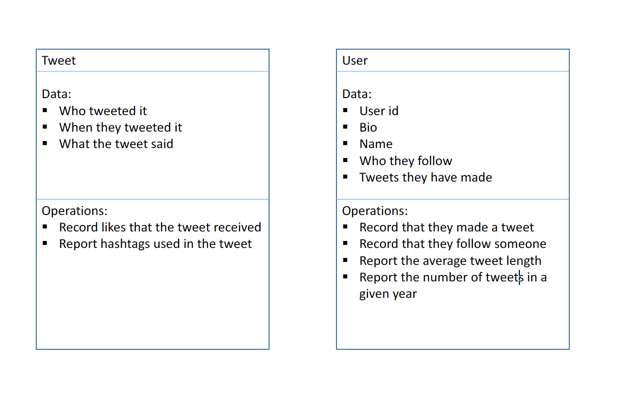
\includegraphics[width=0.8\linewidth]{../images/lab_3/uml.png}
    \end{center}
    \caption{Design for twitter example}
    \label{fig:uml}
\end{figure}

\item You already identified which methods are needed based on your reading of the
starter code.
\item Decide which methods belong in which class and add them to the appropriate
spot in your diagram.
\item What information must be stored in order in order for these methods to provide
their services?
\item Don’t worry about attribute names or types yet, just describe the information
in plain English.
\item Decide which pieces of information belong in which class and add them to the
appropriate spot in your diagram.
\end{enumerate}

\bigskip

\section*{5) Write class \textit{Player}}

\bigskip

Now write the abstract class \textit{Player}. You will probably be able to implement
some methods completely. Other methods you won’t be able to complete at all—they
are abstract. In those methods, the body should simply say

\bigskip

\begin{lstlisting}[language=Python]
    raise NotImplementedError
\end{lstlisting}

\bigskip

\noindent Be sure to include a complete class docstring.

\bigskip

\noindent (You can look at class \textit{NumberGame} for a reminder of what they look like.)
Your docstring should warn that the \textit{Player} class is abstract and should
not be instantiated.

\bigskip

\noindent You do not need to include doctest examples.

\bigskip

\section*{6) Implement class \textit{RandomPlayer}}

\bigskip

Now that we have a \textit{Player} class, we need one or more child classes that can complete
its unimplemented method(s).

\bigskip

\noindent Implement class \textit{RandomPlayer} as a subclass of \textit{Player} (review how
to do this if you aren’t sure).

\bigskip

\noindent Any \textit{Player} methods that were not implemented must be overridden here in
class \textit{RandomPlayer}.

\bigskip

\noindent We have imported module \textit{random} for you.
You will find the function \textit{random.randint} handy—if you aren’t sure how
to use it, import it in the Python console and call \textit{help} on it to learn more!

\section*{7) Make the whole thing run}

\bigskip

Even though you only have one kind of player, you can still make the program run.
Fill in the missing part in \textit{make\_player} to so that it creates a RandomPlayer.

\bigskip

\noindent (Later, we’ll let the user choose from among the three types of player.)

\bigskip

\noindent Run your game! It should be fun to watch two random players battle it out.

\bigskip

\noindent There will likely be small glitches to fix, but they will be things like forgetting an argument, and shouldn’t be hard to fix. Read the error messages carefully—they include very precise information about what’s wrong.

\bigskip

\section*{8) Additional tasks}

\bigskip

If you still have time before this week’s quiz, you can work on the following tasks.

\bigskip

\subsection*{A user player}

\bigskip

\noindent Implement \textit{UserPlayer}. This class takes input from the \textit{User} to
select a move. Recall that you can prompt a user for input by using the built in
\textit{input()} function.

\bigskip

\noindent If you have time, ensure that the user’s moves are legal. But if you are running out of time, don’t bother
with that. It’s not important to the learning goals for this lab.

\bigskip

\noindent Once you have \textit{UserPlayer} done, update \textit{make\_player}
so it gives the user a choice between the two kinds of player that you have
implemented. You'll want to use input() again for this!

\bigskip

\noindent Try playing your game with one user player and one random player. We
hope you can beat the random player!

\bigskip

\subsection*{A strategic player}
Next, add class StrategicPlayer.

\bigskip

\noindent If you haven’t figured out a winning strategy yet, discuss it with some other students.
You should be able to figure out a strategy for the game with goal 21, minimum move 1
and maximum move 3 that will guarantee you win if you go first.

\bigskip

\noindent Even if you go second, if your opponent makes a poor choice you can guarantee a win.

\bigskip

\noindent If you have that “21-1-3” version of the game figured out, try generalizing
the strategy to work for any goal, minimum and maximum.

\bigskip

\noindent (How should you design the code if you can only offer a StrategicPlayer for the 21-1-3 version of the game?)

\bigskip

\noindent Once you have StrategicPlayer implemented, update \textit{make\_player} one last time to give the user the choice of this third kind of player. Try running the game with a strategic and a random player.
Does the strategic one always win?

\bigskip

\subsection*{Tracking and reporting a player’s record}
Because our program allows many rounds of the game to be played, it would be nice to track the record of each player: how many games the player has played, and how many of those games they won.

\noindent Add to your code to keep track of this information, using new attributes on the Player class to do so.

\bigskip

\noindent Then, add a method to the Player class to report the player’s name and record. But there’s a twist! Rather than calling the method like so:

\bigskip

\begin{lstlisting}[language=Python]
    print(p1.report())
\end{lstlisting}

\bigskip

wouldn’t it be nice to say just:

\bigskip

\begin{lstlisting}[language=Python]
    print(p1)
\end{lstlisting}

\bigskip

\noindent In fact you can! If you name a method \_\_str\_\_ and make it return a string, Python will automatically call it whenever
you ask to print an object of this type. \_\_str\_\_ is one of Python’s “special methods.”

\bigskip

\noindent These are methods that you can call using special syntax or built-in functions like print rather than the usual dot notation.

\bigskip

\subsection*{Even more strategies}
Try to generalize your StrategicPlayer to work when there are more than two players. Is this even possible?! Read more about the classic game this lab is based on \href{https://en.wikipedia.org/wiki/Nim}{here} .

\end{document}
